% !TEX TS-program = pdflatex
% !TEX encoding = UTF-8 Unicode

\documentclass[a4paper, titlepage=false, parskip=full-, 10pt]{scrartcl}

\usepackage[utf8]{inputenc}
\usepackage[T1]{fontenc}
\usepackage[english, ngerman]{babel}
\usepackage{babelbib}
\usepackage{hyperref}
\usepackage{listings}
\usepackage{framed}
\usepackage{color}
\usepackage{graphicx}
\usepackage[normalem]{ulem}
\usepackage{cancel}
\usepackage{amsmath}
\usepackage{amssymb}
\usepackage{amsthm}
\usepackage{algorithm}
\usepackage{algorithmic}
\usepackage{geometry}
\usepackage{subfigure}
\geometry{a4paper, top=20mm, left=35mm, right=25mm, bottom=40mm}

\newcounter{tasknbr}
\setcounter{tasknbr}{1}
\newenvironment{task}[1]{{\bf Aufgabe \arabic {tasknbr}\stepcounter{tasknbr}} (#1):\begin{enumerate}}{\end{enumerate}}
\newcommand{\subtask}[1]{\item[#1)]}

% Listings -----------------------------------------------------------------------------
\definecolor{red}{rgb}{.8,.1,.2}
\definecolor{blue}{rgb}{.2,.3,.7}
\definecolor{lightyellow}{rgb}{1.,1.,.97}
\definecolor{gray}{rgb}{.7,.7,.7}
\definecolor{darkgreen}{rgb}{0,.5,.1}
\definecolor{darkyellow}{rgb}{1.,.7,.3}
\lstloadlanguages{C++,[Objective]C,Java}
\lstset{
escapeinside={§§}{§§},
basicstyle=\ttfamily\footnotesize\mdseries,
columns=fullflexible, % typewriter font look better with fullflex
keywordstyle=\bfseries\color{blue},
% identifierstyle=\bfseries,
commentstyle=\color{darkgreen},      
stringstyle=\color{red},
numbers=left,
numberstyle=\ttfamily\scriptsize\color{gray},
% stepnumber=5,
% numberfirstline=true,
breaklines=true,
% prebreak=\\,
showstringspaces=false,
tabsize=4,
captionpos=b,
% framexrightmargin=-.2\textwidth,
float=htb,
frame=tb,
frameshape={RYR}{y}{y}{RYR},
rulecolor=\color{black},
xleftmargin=15pt,
xrightmargin=4pt,
aboveskip=\bigskipamount,
belowskip=\bigskipamount,
backgroundcolor=\color{lightyellow},
extendedchars=true,
belowcaptionskip=15pt}

%% Enter current values here: %%
\newcommand{\lecture}{Algorithmische Geometrie SS15}
\newcommand{\tutor}{}
\newcommand{\assignmentnbr}{4}
\newcommand{\students}{Julius Auer, Alexa Schlegel}
%%-------------------------------------%%

\begin{document}  
{\small \textsl{\lecture \hfill \tutor}}
\hrule
\begin{center}
\textbf{Übungsblatt \assignmentnbr}\\
[\bigskipamount]
{\small \students}
\end{center}
\hrule

\begin{task}{Bewegungsplanung in der Ebene}\item[]
Gegeben sei ein kreisförmiger Roboter $R$ mit Radius $d$, sowie eine Menge $H={p_1, \dots, p_n}$ von $n$ punktförmigen Hindernissen in der Ebene. Eingabewerte sind Startpunkt $s$ und Zielpunkt $z$. Die Ausgabe ist kollisionsfreier Weg $w$ (Polygonzug), falls er existiert, sonst $\emptyset$.

Die Idee des Algorithmus ist es, aus $H$ ein Voronio-Diagramm (VD) zu erstellen und das Zentrum des Roboters auf den Voronio-Kanten (VK) entlang zum bewegen. Zusätzlich werden diejenigen VK entfernt, wo der Abstand der zugehörigen Punkte kleiner ist als der Durchmesser des Roboter. Auf den verbleibenden Kanten kann sich der Roboter bewegen, d.h. sein Zentrum bewegt sich.

Der Algorithmus wird in 3 Schritte unterteilt:

{\large\textcircled{\small{1}}} Roboter von $s$ zum/auf VD bewegen\\
{\large\textcircled{\small{2}}} Roboter entlang des VD bewegen\\
{\large\textcircled{\small{2}}} Roboter von VD zu $z$ bewegen\\

\begin{algorithm}
\caption{movingAround($H, s, z, d$)}
\begin{algorithmic}[1]
\STATE Berechnung VD($H$)
\STATE VR($s$) und VR($z$) bestimmen
\IF{$s$ bzw. $z$ kollidieren mit Punkt in VR($s$) bzw. VR($z$)}
		\RETURN{$\emptyset$}
\ENDIF
\STATE $s'$ und $z'$ auf VD finden und als Knoten zu VD($H$) hinzufügen und Kanten aufsplitten (senkrecht vom Punkt in zugehöriger VR wegbewegen bis VK getroffen wird, siehe~Abbildung\ref{fig:vds})
\STATE Sei $G$ der zugehörige Graph zum VD($H$): alle Kanten entfernen, wo der Abstand der zugehörigen Punkte $\leq d$ ist
\IF{Weg $w$ von $s'$ nach $z'$ existiert}
		\RETURN{$w \cup \overline{ss'} \textrm{ und } \overline{pp'}$}
		\ELSE
				\RETURN {$\emptyset$}
\ENDIF
\end{algorithmic}
\end{algorithm}

\begin{figure}[h]
\begin{center}
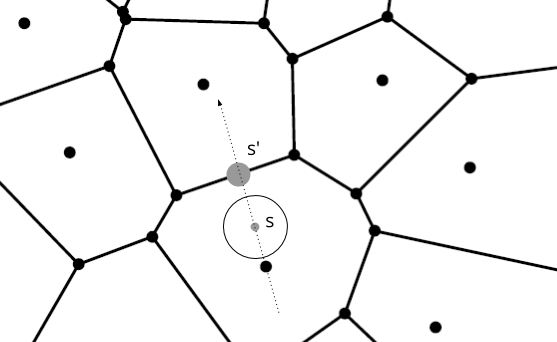
\includegraphics[width=7cm]{vds.png}
\end{center}
\caption{Finden von $s'$}
\label{fig:vds}
\end{figure}

Der existierende Weg kann z.B. per Tiefensuche oder Dijkstra bestimmt werden. Liegt der Start bzw. Endpunkt auf einer Kante die später entfernt wird, so liefert die Suche nach einem existierenden Weg kein Ergebnis.

Was mir noch nicht ganz klar ist, wenn $s$ und $z$ in einer unbeschränkten VR liegen (bzw. man da immer irgendwie hin kommt) dann könnte man doch immer einmal komplett außen rum laufen, oder? Oder ist man in einem Zimmer gefangen wo die Punkte auf dem Boden rumliegen und man sonst gegen die Wand läuft?
\end{task}

\begin{task}{Geometrische Graphen}
\subtask{a}
Induktion über $|V|$:

I.A.: Für $G_1=(V,E,F)$ zusammenhängend und planar mit $|V|=1$ folgt offensichtlich $|E|=0$ und $|F|=1$.

I.V.: Für $G_n=(V,E,F)$ zusammenhängend und planar mit $|V|=n$ gilt: $|E|=|V|+|F|-2$

$n\rightarrow n+1$: Aus $G_{n+1}=(V',E',F')$ zusammenhängend und planar mit $|V'|=n+1$ werden ein Knoten $v$ und alle zu $v$ inzidenten Kanten entfernt. Der entstehende Graph muss nicht zusammenhängend sein. Unabhängig von der Anzahl der Zusammenhangskomponenten (ZHKs) lässt sich aus den folgenden Beobachtungen $|F'|$ ableiten:

{\large\textcircled{\small{1}}} $G_{n+1}$ ohne $v$ und die zu $v$ inzidenten Kanten besteht aus $k\le deg(v)$ planaren ZHKs $G^1,...,G^k$. Für jede ZHK gilt die I.V..\\
{\large\textcircled{\small{2}}} Für das Verbinden dieser ZHKs waren zuvor $k$ Kanten erforderlich, die keine Facetten begrenzten (sonst hätte es einen Kreis und nicht mehrere ZHKs gegeben). Die anderen $deg(v)-k$ Kanten bildeten $deg(v)-k$ Facetten (durch das Hinzufügen zu einer bestehenden ZHK muss ein Kreis und somit eine neue Facette entstehen).\\
{\large\textcircled{\small{3}}} Ferner ist klar, dass sich die $k$ ZHKs eine Facette (die ''Äußere'') teilen - also bei {\large\textcircled{\small{1}}} $k-1$ Facetten zuviel gezählt werden.\\
Somit ergibt sich insgesamt für $|F'|$:
\begin{align*}
|F'|&=\overbrace{\sum_{i=1}^k|F^i|}^{\large\textcircled{\small{1}}}+\overbrace{(deg(v)-k)}^{\large\textcircled{\small{2}}}-\overbrace{(k-1)}^{\large\textcircled{\small{3}}}\\
&=\sum_{i=1}^k(|E^i|-|V^i|+2)+deg(v)-2\cdot k+1\\
&=|E'|-deg(v)-(|V'|-1)+2\cdot k+deg(v)-2\cdot k+1\\
&=|E'|-|V'|+2\\
\end{align*}
\qed

\subtask{b}
Sei $D$ die Menge der Dreiecke des triangulierten Graphen $G=(V,E)$. $r$ Knoten liegen auf dem Rand der konvexen Hülle der Punkte aus $G$ und beschreiben einen geschlossenen Polygonzug, der folglich aus ebenfalls $r$ Kanten $E_r$ besteht. Jede dieser Kanten grenzt an genau ein Dreieck. Die $|E|-|E_r|$ Kanten, die im Inneren des Graphen liegen, begrenzen jeweils zwei Dreiecke. Jedes Dreieck wiederum wird von drei Kanten begrenzt. Somit gilt:
\begin{align*}
&|E_r|+2\cdot (|E|-|E_r|)=3\cdot |D|\\
\Leftrightarrow &|E|=\frac{3\cdot |D|+r}{2}
\end{align*}
In (a) wurde gezeigt, dass:
$$|F|=|E|-|V|+2$$
Wobei hier offensichtlich $|D|=|F|-1$ (die ''äußere'' Facette ist kein Dreieck). Das sollte ausreichen, etwas Aussagekräftiges auszurechnen :)
\begin{align*}
|F|&=|E|-|V|+2\\
\Leftrightarrow |D|+1&=\frac{3\cdot |D|+r}{2}-n+2\\
\Leftrightarrow |D|&=2\cdot n-r-2\\
&=2\cdot (n-1)-r
\end{align*}
\qed
\end{task}

\begin{task}{Voronoi-Diagramm}\item[]
Das dürfte straight-forward funktionieren:

Eingabe ist ein Voronoi-Graph mit Knoten $V$, Kanten $E$ und Facetten $F$ sowie die leere Menge $CH$ die nach aufruf von $CH(V,E,F,CH)$ die konvexe Hülle von $S$ enthält. Für eine Kante $e$ seien $e.f1$ und $e.f2$ die angenzenden Facetten. Für eine Facette $f$ seien $E(f)$ die angrenzenden Kanten.

\begin{algorithm}
\caption{$CH(V,E,F,CH)$}
\begin{algorithmic}[1]
\STATE$start:=\text{Facette mit minimaler x-Koordinate}$\\
\STATE$f:=start$\\
\STATE$last:=null$
\REPEAT
\STATE$CH\leftarrow f$\\
\FOR{$\text{ \bf each }e\in E(f)$}
\IF{$e\text{ is unbound }$\AND\NOT$(e.f1=last$ \OR$e.f2=last)$}
\STATE$last:=f$\\
\STATE$f:=(f=e.f1?e.f1:e.f2)$\\
\STATE$\text{\bf break}$
\ENDIF
\ENDFOR
\UNTIL{$r=start$}
\end{algorithmic}
\end{algorithm}

Es wird auf den äußeren Facetten entlanggelaufen, bis man wieder den Ausgangspunkt erreicht. Hierfür überquert man immer genau die Kante von der man nicht gekommen ist, und die ein offenes Ende hat.

(1) benötigt $O(n)$ Zeit.\\
(4) wird $O(n)$ mal wiederholt\\
(6-12) kann zwar $O(n)$ mal wiederholt werden, insgesamt wird jedoch offensichtlich in (4-13) jede äußere (ungebundene) Kante nur konstant oft betrachtet. Die Anzahl Kanten ist asymptotisch begrenzt durch die Anzahl der Knoten, womit insgesamt keine Kosten von mehr als $O(n)$ zu erwarten sind.

Insgesamt ist ein Zeitaufwand von $O(n)$ zu erwarten, zusätzlicher Speicherplatz ist nicht erforderlich ($O(n)$ für die konvexe Hülle).
\end{task}
\end{document}